\documentclass{beamer}
\usepackage[utf8]{inputenc}
\usepackage[english,german]{babel} 
\usepackage{listings} 
\usepackage{listings-golang}

\usepackage[absolute,overlay]{textpos}
  \setlength{\TPHorizModule}{1mm}
  \setlength{\TPVertModule}{1mm}

\titlegraphic{
\includegraphics[scale=0.1]{golanglogo.png}}
\title{
	\Large{\textit{\\Die Programmiersprache Go - Eine Einf\"uhrung}} \\
	\Large{\textbf{\\Seminarvortrag}}
}
\author{Student: Adrian Helberg \\Prüfer: Prof. Dr. Axel Schmolitzky}
\date{\today}

\definecolor{mygreen}{rgb}{0,0.6,0}

\begin{document}
\lstset{
    frame=single,
    basicstyle=\footnotesize,
    keywordstyle=\color{blue},
    showstringspaces=false, 
    stringstyle=\color{mygreen},
    tabsize=4,
    language=Golang
}

\maketitle

\frame{\tableofcontents}

\begin{frame}

\begin{quote}
``Go is an open source programming language that makes it easy to build simple, reliable and efficient software." 
\end{quote}

\begin{flushright}
\scriptsize (Go Website: \href{golang.org}{golang.org})
\end{flushright}

\begin{quote}
Go ist eine Open-Source-Programmiersprache, die es einfach macht, einfache, zuverlässige und effiziente Software zu erstellen.
\end{quote}

\begin{flushright}
\scriptsize (Eigene \"Ubersetzung)
\end{flushright}

\end{frame}

\section{Geschichte}
\subsection{Entwickler}
\begin{frame}
\frametitle{Entwickler}

\begin{itemize}
\setlength{\itemsep}{24pt}
\item Konzipiert September 2007
\item Robert Griesemer, Rob Pike und Ken Thompson
\item Mitarbeiter von Google LLC \textregistered
\item Aus Frust heraus entstanden
\item \textit{``Complexity is multiplicative''} - Rob Pike
\end{itemize}

\end{frame}

\subsection{Entwurfsphase}
\begin{frame}
\frametitle{Entwurfsphase}

\begin{itemize}
\setlength{\itemsep}{40pt}
\item Ausdrucksstarke und effiziente Kombination aus Kompilierung und Ausf\"uhrung
\item Ähnlichkeiten mit C
\item Adaptiert gute Ideen aus einigen Programmiersprachen: \\
Pascal, Modula-2, Oberon, Oberon-2, Alef, ...
\end{itemize}

\end{frame}

\begin{frame}
\frametitle{Entwurfsphase}

\begin{figure}
\centering
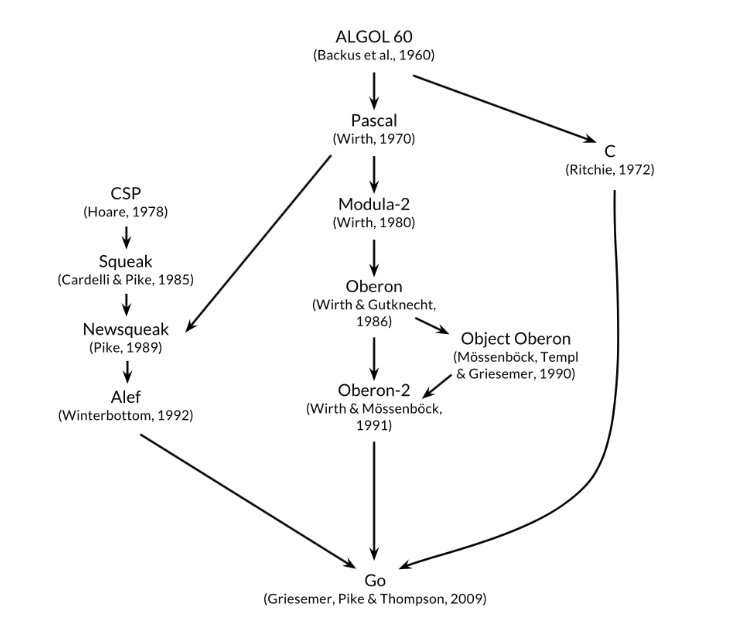
\includegraphics[scale=0.45]{origin.png}
\caption{The Go Programming Language,  Preface xii}
\end{figure}

\end{frame}

\begin{frame}
\frametitle{Entwurfsphase}

\begin{itemize}
\setlength{\itemsep}{40pt}
\item Vermeiden von features, die zu komplexen, unzuverl\"assigen code führen w\"urden
\item M\"oglichkeiten zur Nebenl\"aufigkeit sind neu und effizient
\item Datenabstraktion und Objektorientierung sind ungewohnt flexibel
\item Automatische Speicherverwaltung (garbage collection)
\end{itemize}

\end{frame}

\subsection{Ver\"offentlichung}
\begin{frame}
\frametitle{Ver\"offentlichung}

\begin{itemize}
\setlength{\itemsep}{60pt}
\item Vorgestellt November 2009
\item Ber\"uhmt als Nachfolger für nicht typisierte Sriptsprachen
\begin{itemize}
\item[] $\rightarrow$ Verbindung aus Ausdruckskraft und Sicherheit
\end{itemize}
\end{itemize}

\end{frame}

\subsection{Go-Community}
\begin{frame}
\frametitle{Go-Community}

\begin{itemize}
\setlength{\itemsep}{44pt}
\item Open-source projekt
\begin{itemize}
\item[] $\rightarrow$ Quellcode des Compilers, Bibliotheken (libraries) und Tools sind frei verfügbar
\end{itemize}
\item Aktive, weltweite Community
\item L\"auft auf Unix, Mac und Windows
\begin{itemize}
\item[] $\rightarrow$ \"Ublicherweise ohne Modifikation transpotrierbar
\end{itemize}
\end{itemize}

\end{frame}

\section{Merkmale}

\subsection{Einsatzbereich}
\begin{frame}
\frametitle{Einsatzbereich}

\begin{itemize}
\item ``Alles was auf dem Server l\"auft''
\item \"Okosystem
\item vorhendene Libraries und Projekte
\end{itemize}

\end{frame}

\begin{frame}

\begin{itemize}
\setlength{\itemsep}{16pt}
\item Reflection
\item Typsicherheit
\item Autmoatische Speicherbereinigung
\item Interfaces, Mixins $\rightarrow$ Objektorientierung
\item Keine Klassen $\rightarrow$ Java Vergleich
\item Pakete
\end{itemize}

\end{frame}

\begin{frame}

\frametitle{Projekte}

\begin{textblock}{20}(10,30)
\textit{Go}

\includegraphics[scale=0.22]{docker.png}
\end{textblock}

\begin{textblock}{20}(60,32)
\textit{Java}

\includegraphics[scale=0.22]{elasticsearch.png}
\end{textblock}

\end{frame}

\section{Syntax}
\begin{frame}[fragile]
\frametitle{Syntax}

%%% GO
Go
\begin{lstlisting}
package main

import "fmt"

func main() {
    fmt.Println("Hello World!")
}
\end{lstlisting}

%%% JAVA
Java
\lstset{language=Java}
\begin{lstlisting}
public class HelloWorld 
{ 
    public static void main (String[] args)
    {
        System.out.println("Hello World!");
    }
}
\end{lstlisting}

\end{frame}

\section{Paradigmen}
\begin{frame}
\frametitle{Paradigmen}

\begin{itemize}
\setlength{\itemsep}{20pt}
\item Nebenläufig
\item Imperativ
\item Strukturiert
\item Modular
\item Objektorientiert
\end{itemize}

\end{frame}

\section{Zentrale Fragestellung}
\begin{frame}
\frametitle{Zentrale Fragestellung}

\centering
\glqq flexibel wie dynamisch getyped,\\ aber mit statischer Typsicherheit?\grqq{}

\end{frame}

\section{Pro \& Contra}
\begin{frame}
\frametitle{Pro \& Contra}

\begin{tabular}{p{5cm} | p{5.5cm}}
\textbf{Pro} & \textbf{Contra} \\ \hline
\begin{itemize}
\setlength{\itemsep}{20pt}
\item Minimalismus
\item Statisches Duck-Typing
\item Parallelisierung
\item Aufger\"aumte Syntax
\item Schneller Compiler
\end{itemize}
&
\begin{itemize}
\setlength{\itemsep}{20pt}
\item Keine generische Programmierung
\item nil statt Option
\item Wenig grundlegende Datenstrukturen
\item Keine Methodenüberladung
\end{itemize}
\\
\end{tabular}

\end{frame}

\begin{frame}
\frametitle{Pro \& Contra}

\begin{tabular}{p{5cm} | p{5.5cm}}
\textbf{Pro} & \textbf{Contra} \\ \hline
\begin{itemize}
\setlength{\itemsep}{20pt}
\item Statisch gelinkte Binärdateien
\item Laufzeiteigenschaften
\item Integriertes Unit-Test-Framework
\item Paketmanager
\end{itemize}
&
\begin{itemize}
\setlength{\itemsep}{20pt}
\item Unbefriedigende API-Dokumentation
\item Teilweise umständliche APIs
\item Umst\"andliches Mocking
\item Kleines \"Okosystem
\end{itemize}
\\
\end{tabular}

\end{frame}

\section{Compiler}
\begin{frame}
\frametitle{Compiler}

\begin{itemize}
\setlength{\itemsep}{20pt}
\item Gc
\item Gccgo
\end{itemize}

\end{frame}

\section{Einzelnachweise}
\begin{frame}
\frametitle{Einzelnachweise}

\begin{itemize}
\setlength{\itemsep}{20pt}
\item ...
\end{itemize}

\end{frame}

\end{document}